\chapter{Background and Related Work}


\section{Background}
In this section, we will discuss about different types 360 videos, then about the system level overview and the data flow within the system. We provide some necessary background to understand the image stitching pipeline by visually showing the intermediate outputs. 

\subsection{Types of 360 degree videos}
There are mainly ways three types of 360 capturing viz, monoscopic, Omni-directional Stereo(ODS), and Light Field cameras. In this work we will focus on monoscopic and stereoscopic cameras. 
\subsubsection{Monoscopic 360 Degree}
Fisheye lenses allow image sensors to capture images within an ultra-wide hemispheric field of view. With two fisheye-lensed sensors that capture complementary fields of view each of over 180\textdegree , the pair of captured images can be processed to achieve over a spherical 360\textdegree  x 180\textdegree  area, as shown in \ref{fig:Mono} The equirectangular projection format is a common format for 360\textdegree  x 180\textdegree  images, allowing remapping to other projections for convenient viewing. To create equirectangular images, the paired fisheye capture data  goes though multiple stage, Viz, Projection Mapping, Correspondence(optical flow), view synthesis, and compression.
\begin{figure}[h]
	\centering
	\begin{subfigure}{.5\textwidth}
		\centering
		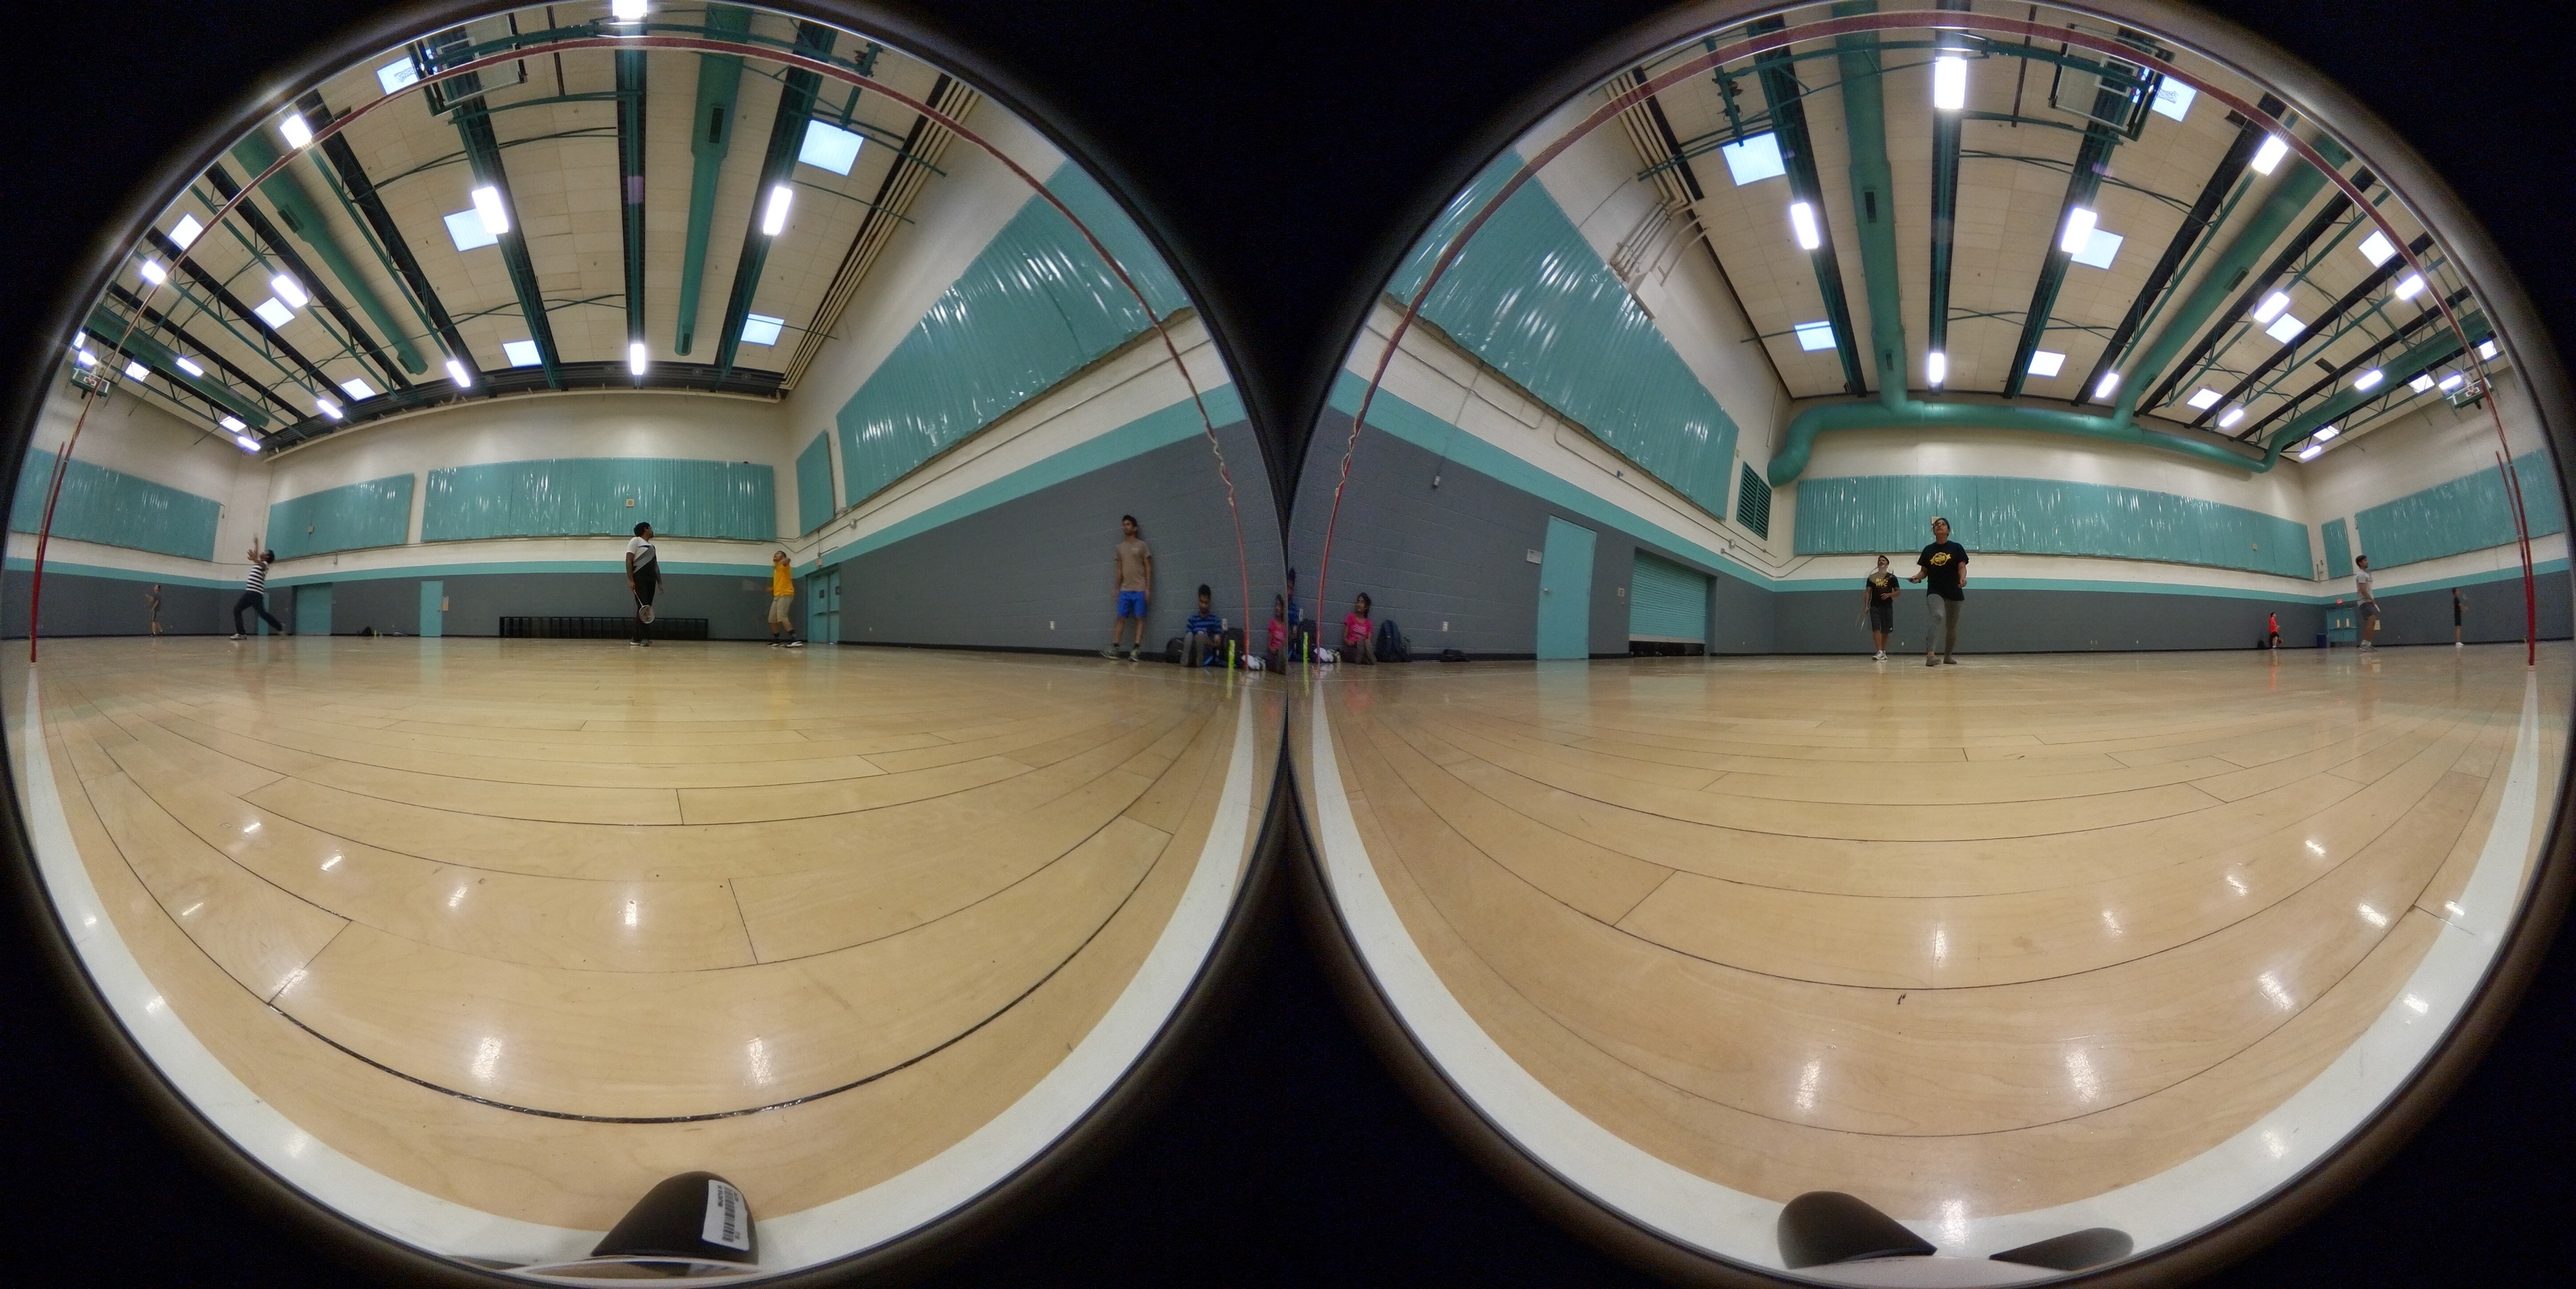
\includegraphics[width=1\linewidth]{/media/gunman/Data/thesis/ThesisLatex/data/images/fisheye_image_pair.jpg}
		\caption{Pair of spherical fisheye images}
		\label{fig:Mono input}
	\end{subfigure}%
	\begin{subfigure}{.5\textwidth}
		\centering
		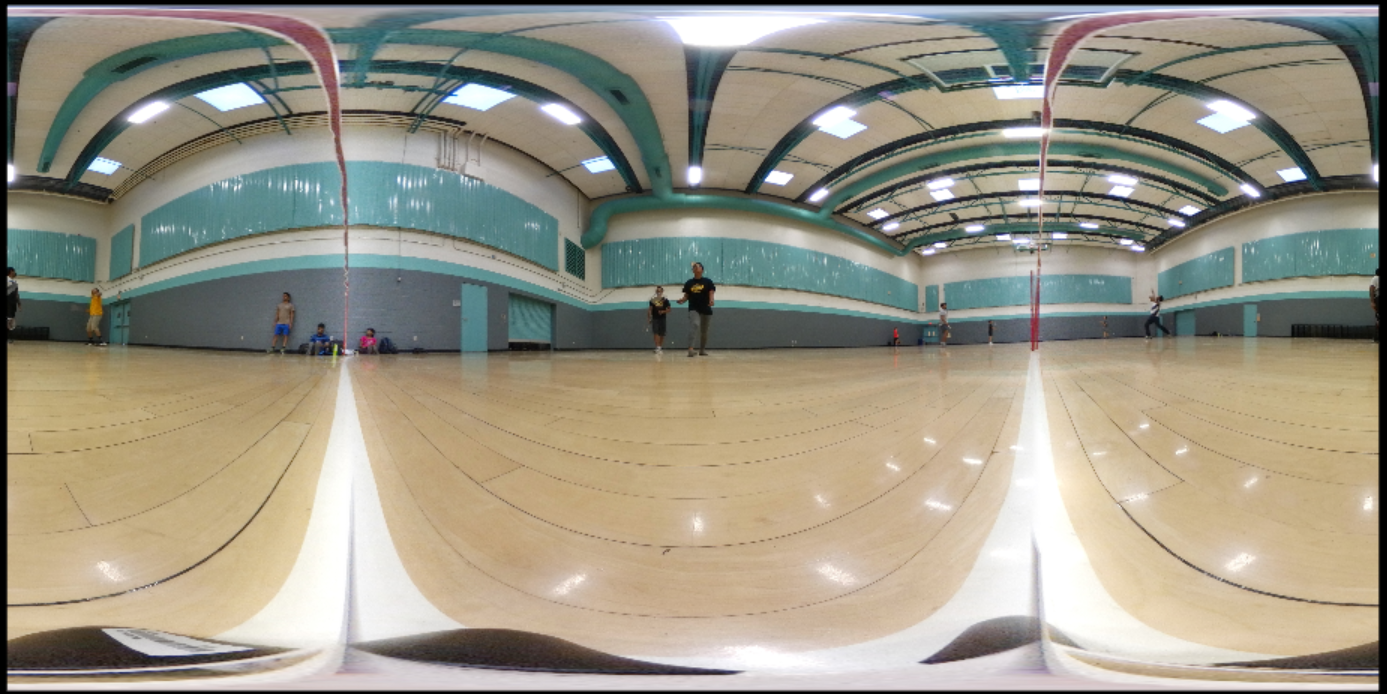
\includegraphics[width=1\linewidth]{/media/gunman/Data/thesis/ThesisLatex/data/images/fisheye_2_equirect.png}
		\caption{Equirectangular projected output}
		\label{fig:Mono Output}
	\end{subfigure}
	\caption{A 360 degree capture and corresponding panorama}
	\label{fig:Mono}
\end{figure}



\subsubsection{Omni-directional Stereo(ODS)}
ODS output consist of two panoramas one for each eye, and provide the binocular stereo needed for perceiving depth information of the scene with respect to the view point of capturing device. In order to generate such output, we need to capture stereo information from all the viewing directions. Instead of capturing from all the viewing directions, we capture in certain directions, equally distributed over the 360 degree viewing angle and later process them to get the virtual camera viewpoints. We finally get the two panoramas one for each eye, which helps see the 360 view with depth. The inputs and outputs can be seen in \ref{fig:ODS_IO}.




\begin{figure}[h]
	\begin{center}
		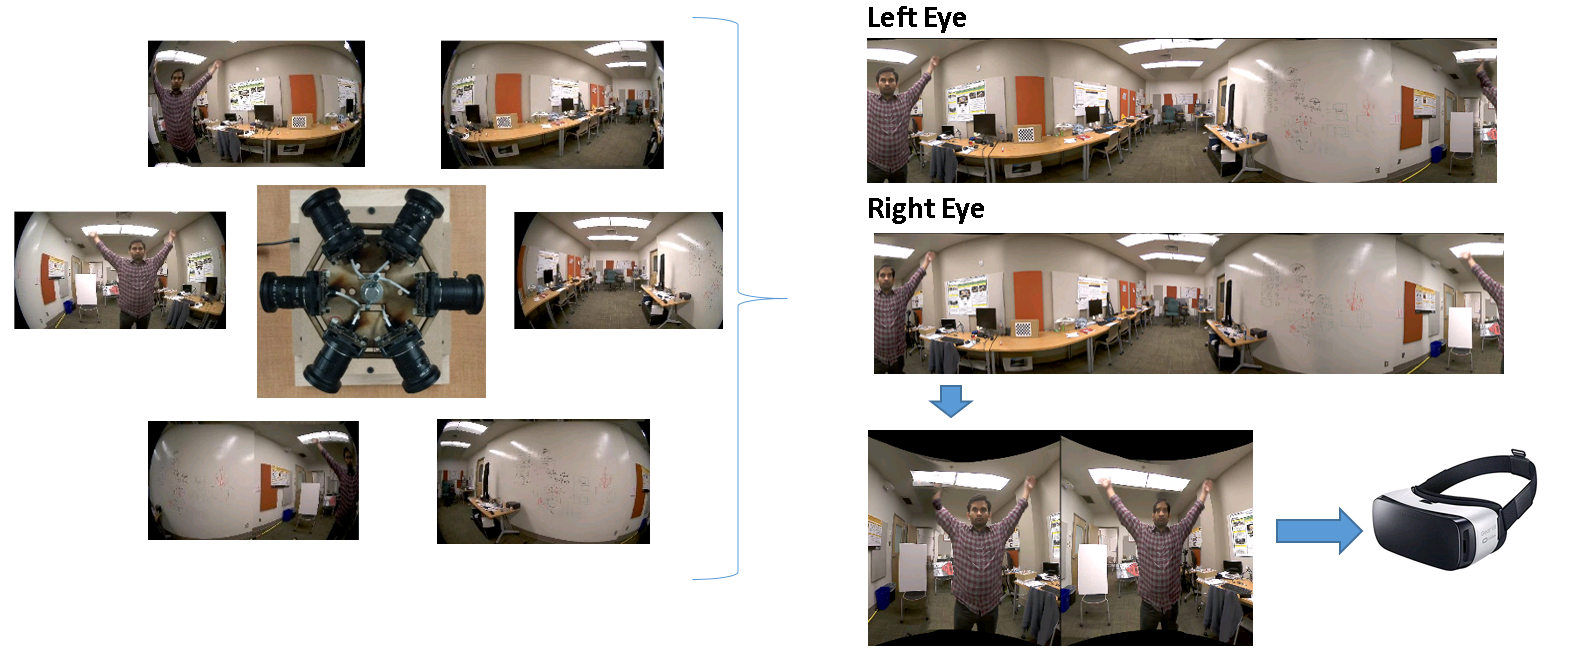
\includegraphics[width=1\textwidth]{/media/gunman/Data/thesis/ThesisLatex/data/images/ODS_IO_images.png}
	\end{center}
		\caption{Left side of the picture shows the multi-view point capture and the right side shows the two ODS panorama, one for each eyes.}	
\label{fig:ODS_IO}
\end{figure} 

\subsection{Stages in ODS Stitching}
The inputs of the ODS system are fisheye images and the outputs are two stereo panoramas. We will need multiple view points so that we can capture both in 360 and in depth. But at high level both for monoscopic and stereoscopic we need to go though the same stages for generating output viz., Projection Mapping, Correspondence, blending, compression.
\subsubsection{Projection Mapping}The equirectangular images as shown in \ref{fig:ODS_Proj} are populated by sourcing image pixels from the fisheye images along a (spherical coordinate to polar coordinate) projection map. As projected pixel coordinates typically fall between integer pixel coordinates, the algorithm typically either pulls a nearest-neighbor pixel or a bilinear combination of a neighborhood of pixels. 
\begin{figure}[h]
	\begin{center}
		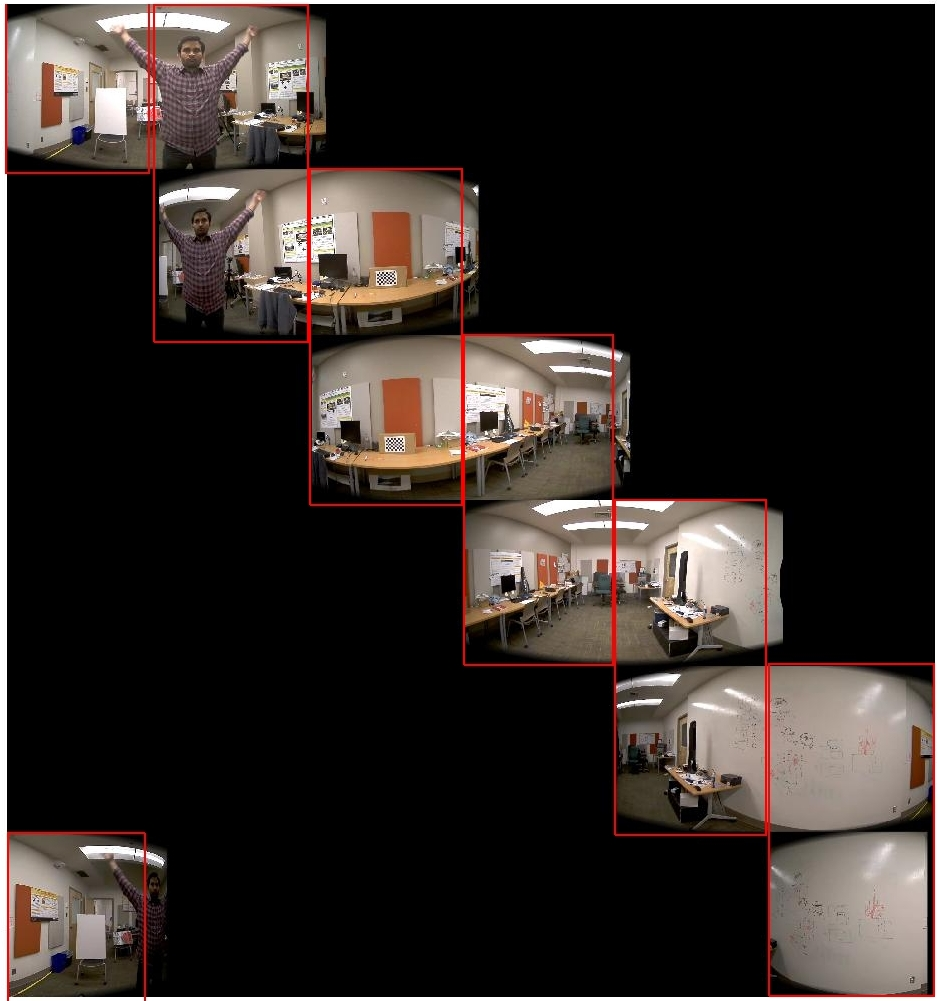
\includegraphics[width=0.5\textwidth]{/media/gunman/Data/thesis/ThesisLatex/data/images/EqRect_offset_fov_viz_loop_v3.jpg}
		%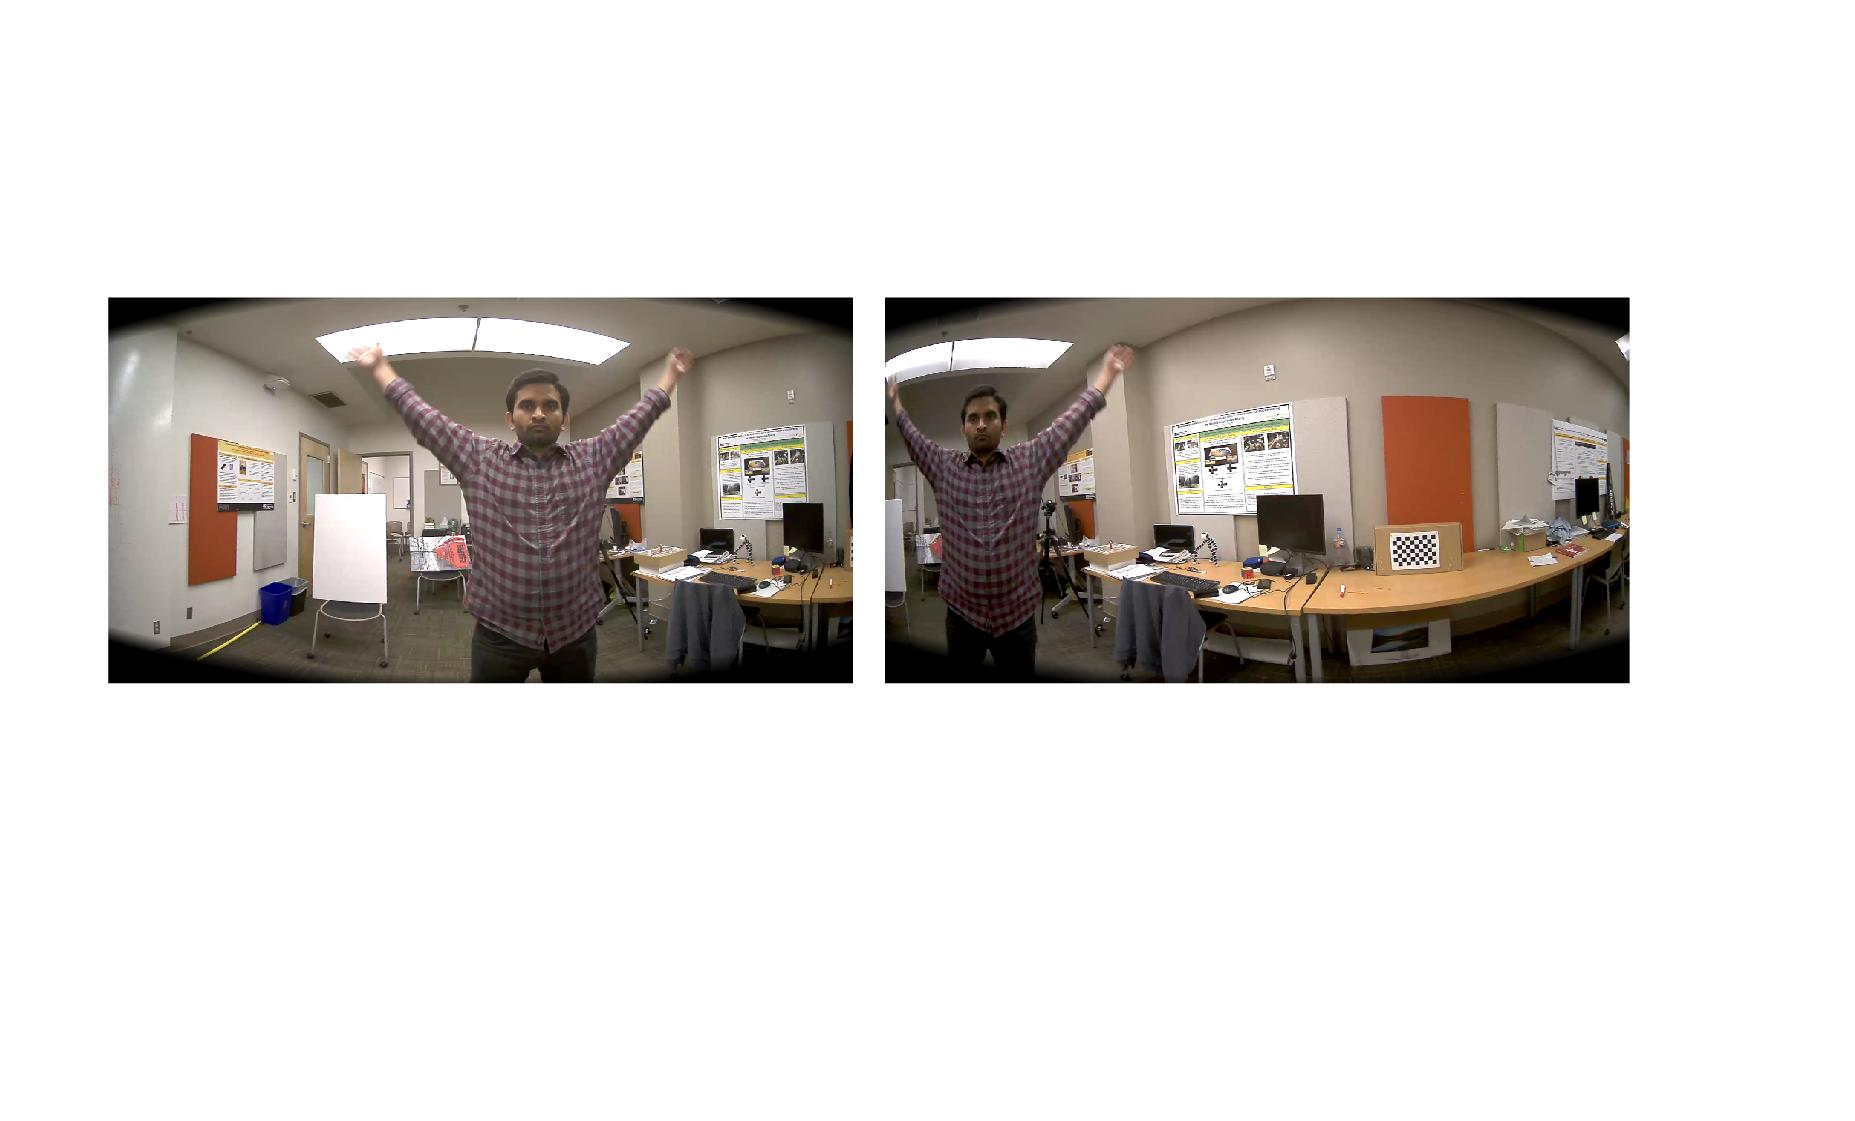
\includegraphics[width=1\textwidth]{/media/gunman/Data/thesis/ThesisLatex/data/images/EqRect_2_adj_images.jpg}
		\caption{Equirectangular Projection of different fisheye images with offsets showing where they belong in the final ODS panorama.}
		\label{fig:ODS_Proj}
	\end{center}
\end{figure} 

\subsubsection{Stereo Correspondence}  As the two fisheye cameras do not precisely occupy the same point in space, objects at the edges of fisheye images appear in different positions in the images, dependent on their distances from the camera. This phenomenon is called the parallax effect. To ensure that objects appear properly, a correspondence algorithm identifies matching visual features across image pairs, warping the projection to reduce object seams in the image. For ODS, we need dense stereo correspondence between the adjacent views to generate novel views as shown in \ref{fig:stereo_disparity}. We generate the stereo correspondence using spatial optical flow, i.e the optical flow between adjacent cameras. The optical flow signifies how far or how near a point is from the capture rig. 
\begin{figure}[h]
	\begin{center}
		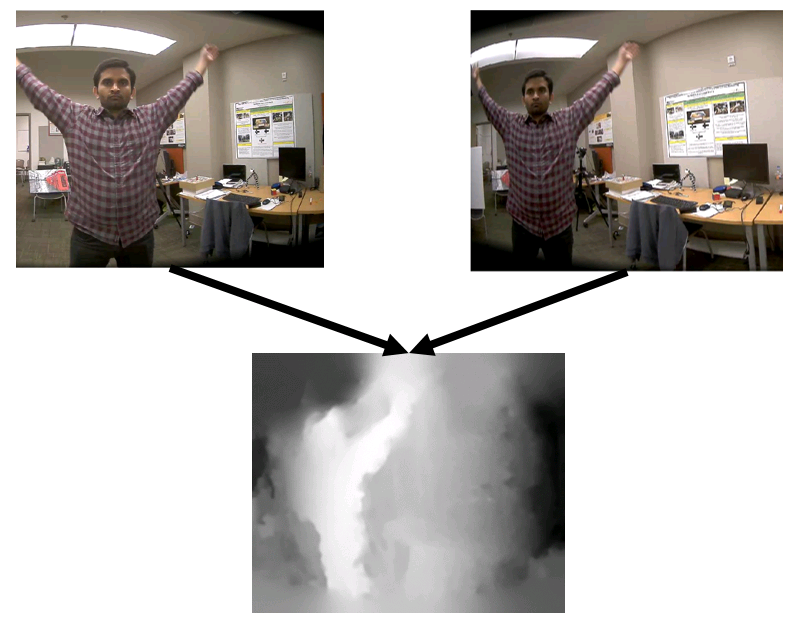
\includegraphics[width=1\textwidth]{/media/gunman/Data/thesis/ThesisLatex/data/images/stereo_disparity.png}		
	\end{center}
	\caption{From the overlapping view of adjacent views, we get stereo disparity, i.e how far each point is away from the camera.}
	\label{fig:stereo_disparity}
\end{figure} 
\subsubsection{View Synthesis}
The ODS needs novel camera views so that it can collect rays from all the directions. But as we have limited number of cameras, we can use these camera views and the dense stereo correspondences to generate the novel views which represent the images taken if there was a camera in between. 
\subsubsection{Blending}  Even after projection and correspondence suggest image overlay coordinates, intensity variations from misalignments still occur between the two projected images at the stitching boundary. The blending stage combines the images through a weighted sum of pixel values to generate a seamless 360\textdegree    image with a smooth transition.	 
\subsubsection{Compression}  To reduce the bandwidth at the capture, networking, or storage interface, images can be compressed into representations that use smaller file sizes. Lossy compression schemes, e.g., JPEG/MPEG, allow dramatic reductions in file size by discarding information that is considered to be perceptibly irrelevant.


\section{System Overview and Data Flow}

The end to end system consist of four main stages viz., image sensor, image signal processor(ISP), processor, and Off-chip memory, as shown in \ref{fig:Sys_overview} The image sensor captures raw images, which are processed by ISP to generate RGB images and the DRAM supports for storage of images and data for all the above stages. The ISP is typically integrated with the processor SoC, and Camera and DRAM are implemented in separate chips.
 
\begin{figure}[h]
	\begin{center}
		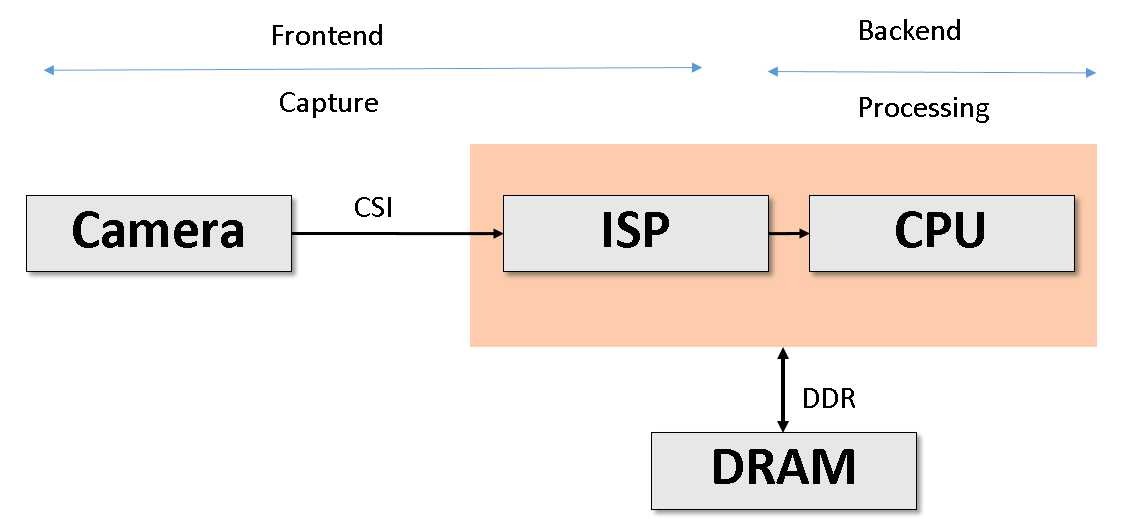
\includegraphics[width=1\textwidth]{/media/gunman/Data/thesis/ThesisLatex/data/images/System_overview.png}
	\end{center}
		\caption{System overview, the Camera, ISP, Processor and Storage.}
\label{fig:Sys_overview}
\end{figure} 

\subsubsection{Hardware}
We have 3 major components, the cameras, the support rig and the evaluation platform. For capture we use six cameras with 2k resolution and 30 fps. The table \ref{Tab:Hardware_Specifications} shows the specs of the cameras used for prototype design. The rig is designed with precision using laser cutting a hard cardboard.  For capturing and computation we use Nvidia Jetson TX2 board.

\subsubsection{Software}
For camera capture we use the libargus camera api provided by Nvidia. For stitching we adapt the facebook surround 360 to work on our platform.
\begin{figure}[h]
	\begin{center}
		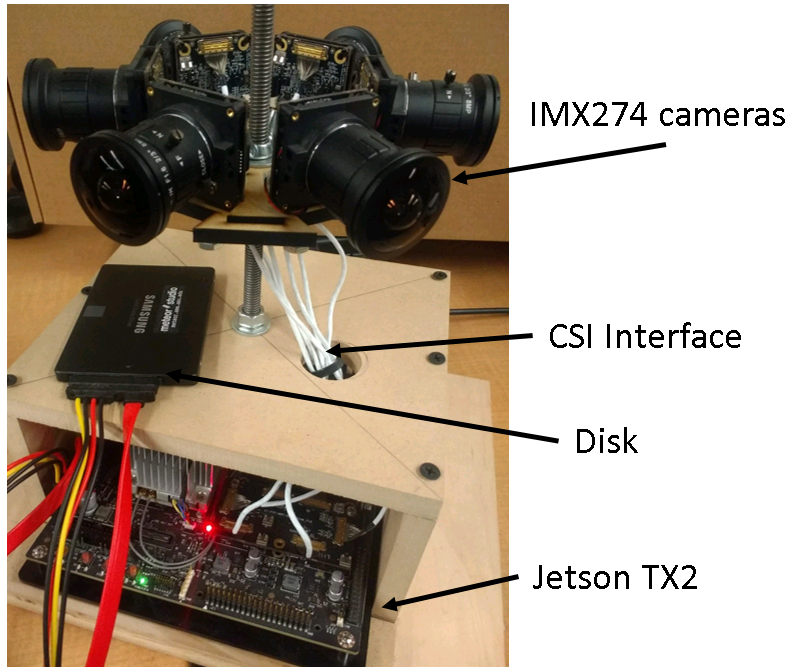
\includegraphics[width=1\textwidth]{/media/gunman/Data/thesis/ThesisLatex/data/images/Prototype.png}
	\end{center}
	\caption{Camera capture rig and the evaluation platform}
	\label{fig:Prototype}
\end{figure} 


\begin{table}[]

	\\\specialrule{2pt}{0pt}{0pt}
\begin{tabular}{!{\VRule[2pt]}c|!{\VRule[2pt]}c!{\VRule[2pt]}}
	
	\textbf{Cameras} &  \\\specialrule{3pt}{0pt}{0pt}
	Type & Sony IMx274 \\\hdashline
	Output Image Size & Diagonal 7.20 mm (Type 1 / 2.5) aspect ratio 16:9 \\\hdashline
	Number of Effective Pixels & 3864 (H) x 2202 (V) approx. 8.51M pixels \\\hdashline
	Unit cell size & 1.62 um (H) x 1.62 um (V) \\\hdashline
		\textbf{Hardware} & \\\specialrule{3pt}{0pt}{0pt}
		Board & Nvidia Jetson TX2\\\hdashline
		CPU & Quad-core ARM A57 \\\hdashline
		ISP & 1200 Million Pix/Sec \\\hdashline
		\textbf{Software} & \\\specialrule{3pt}{0pt}{0pt}
		OS & Ubuntu 16.04 \\\hdashline
		Stitching & Facebook surround 360 \\\hdashline
		Implementation & c++, openCV \\\specialrule{3pt}{0pt}{0pt}
\end{tabular} 
	\caption{Prototype Specifications}
\label{Tab:Hardware_Specifications}
\end{table}


%\subsection{Energy}
%Data and power numbers for Google Jump VR:
%Number of cameras: 17 ; Data Generated per each frame by 17 cameras(in bayer): 816 MB
%
%Data bandwidth requirement in Gb/s : 47.8 Gb/s
%(@30fps, compressed data(1:8 compression ratio))
%
%Power:
%Camera Capture and basic processing at camera:  50 W
%DRAM power(approx.) : 61 W 
%(30 W corresponds to store data generated by 30 frames of all 17 cameras)
%On chip LVDS power(approx): 19 W
%(For transferring one frame of all 17 cameras)
%Compute Power: ( very high, done offline using multiple GPU's)
%Facebook also has 360 stereo solutions, one with 24 cameras and other with 6 cameras. I may need to find data for them as well. Consumes similar amount of power.
%\subsection{Latency}
%Several hours for final ODS generation.
